% !TEX root = ../thesis.tex
After looking at the general feasibility of the Cumlants, we now turn our attention to a standard benchmark in fluid dynamics, Schaefer-Turek,~\cite{schafer1996benchmark}.
There, the authors collected computations for various flows around cylinders and rectangles in $2$ and $3$ spatial dimensions under varying conditions and on different grids.

\begin{figure}
  \centering
  % !TEX root = ../../thesis.tex


\begin{tikzpicture}

\draw[color=gray, style=dashed] (-0.5,2) -- (2,2);
\draw[color=gray, style=dashed] (-0.5,2.5) -- (2,2.5);
\draw[color=gray, style=dashed] (2,-0.5) -- (2,2);

\fill[pattern=north east lines, pattern color=gray] (0,0) rectangle (10,-0.2);
\fill[pattern=north east lines, pattern color=gray] (0,4.1) rectangle (10,4.3);
\draw (0,0) .. controls (1,1.55) and (1,2.55) .. (0,4.1);
\draw (0,0) -- (10,0);
\draw (0,4.1) -- (10,4.1);
\draw (0,0) -- (0,4.1);

\draw[->] (0,4.1/2) -- (0.75,4.1/2);
\draw[->] (0,2.73) -- (0.66,2.73);
\draw[->] (0,1.36) -- (0.66,1.36);
\draw[->] (0,3.4) -- (0.4,3.4);
\draw[->] (0,0.68) -- (0.4,0.68);

\node (u) at (0.3,2.3) {$\vec{u}$};


\draw[->] (-0.5,-0.7) -- (-0.5,5);
\draw[->] (-0.5,-0.7) -- (10.5,-0.7);

\node (y) at (-0.5,5.2) {$y$};
\node (x) at (10.7,-0.7) {$x$};


\node (nullx) at (0,-0.95) {$0$};
\draw[-] (-0.55,0) -- (-0.45,0);

\node[anchor=east] (nully) at (-0.5,0) {$0$};
\draw[-] (0,-0.65) -- (0,-0.75);

\fill[pattern=north east lines, pattern color=gray, draw=black]  (2,2) circle (0.5);

\node at (2,-0.95) {$0.2$};
\draw[-] (2,-0.65) -- (2,-0.75);
\node  at (10,-0.95) {$2.2$};
\draw[-] (10,-0.65) -- (10,-0.75);

\node[anchor=east]  at (-0.5,2) {$0.2$};
\draw[-] (-0.55,2) -- (-0.45,2);

\node[anchor=east]  at (-0.5,2.5) {$0.25$};
\draw[-] (-0.55,2.5) -- (-0.45,2.5);

\node[anchor=east]  at (-0.5,4.1) {$0.41$};
\draw[-] (-0.55,4.1) -- (-0.45,4.1);
\fill[ draw=black]  (2,2) circle (0.02);

\end{tikzpicture}

  \caption{Setup for the Schaefer-Turek benchmark `2D-2'}
\label{fig: schaeferTurek}
\end{figure}

Figure~\ref{fig: schaeferTurek} gives an overview of the problem we examine.
We have a channel flow at a low Reynolds number of $100$, similar to the Poiseuille flow.
This time however, there is a cylinder placed slightly off the vertical center and exposed to the parabolic inflow.
The quantity of interest is the lift it experiences\footnote{Forces are calculated via a momentum exchange, which is independent of the collision we use and thus not elaborated further.}.

Again, a grid study is done, this time controlling the radius of the sphere and scaling the computational domain accordingly to preserve the ratios.
This brings one caveat however:
As we scale our spatial coordinates, we also have to scale our timesteps, according to equation~\eqref{eq: relation between stepsizes}.
Hence, for double the resolution in each of the spatial dimensions, we don't need $4$ times but $8$ times the computation time to cover the same simulated time.
Thus, any savings in spatial resolution will pay off greatly in the final computation times.


\begin{figure}
  \centering
  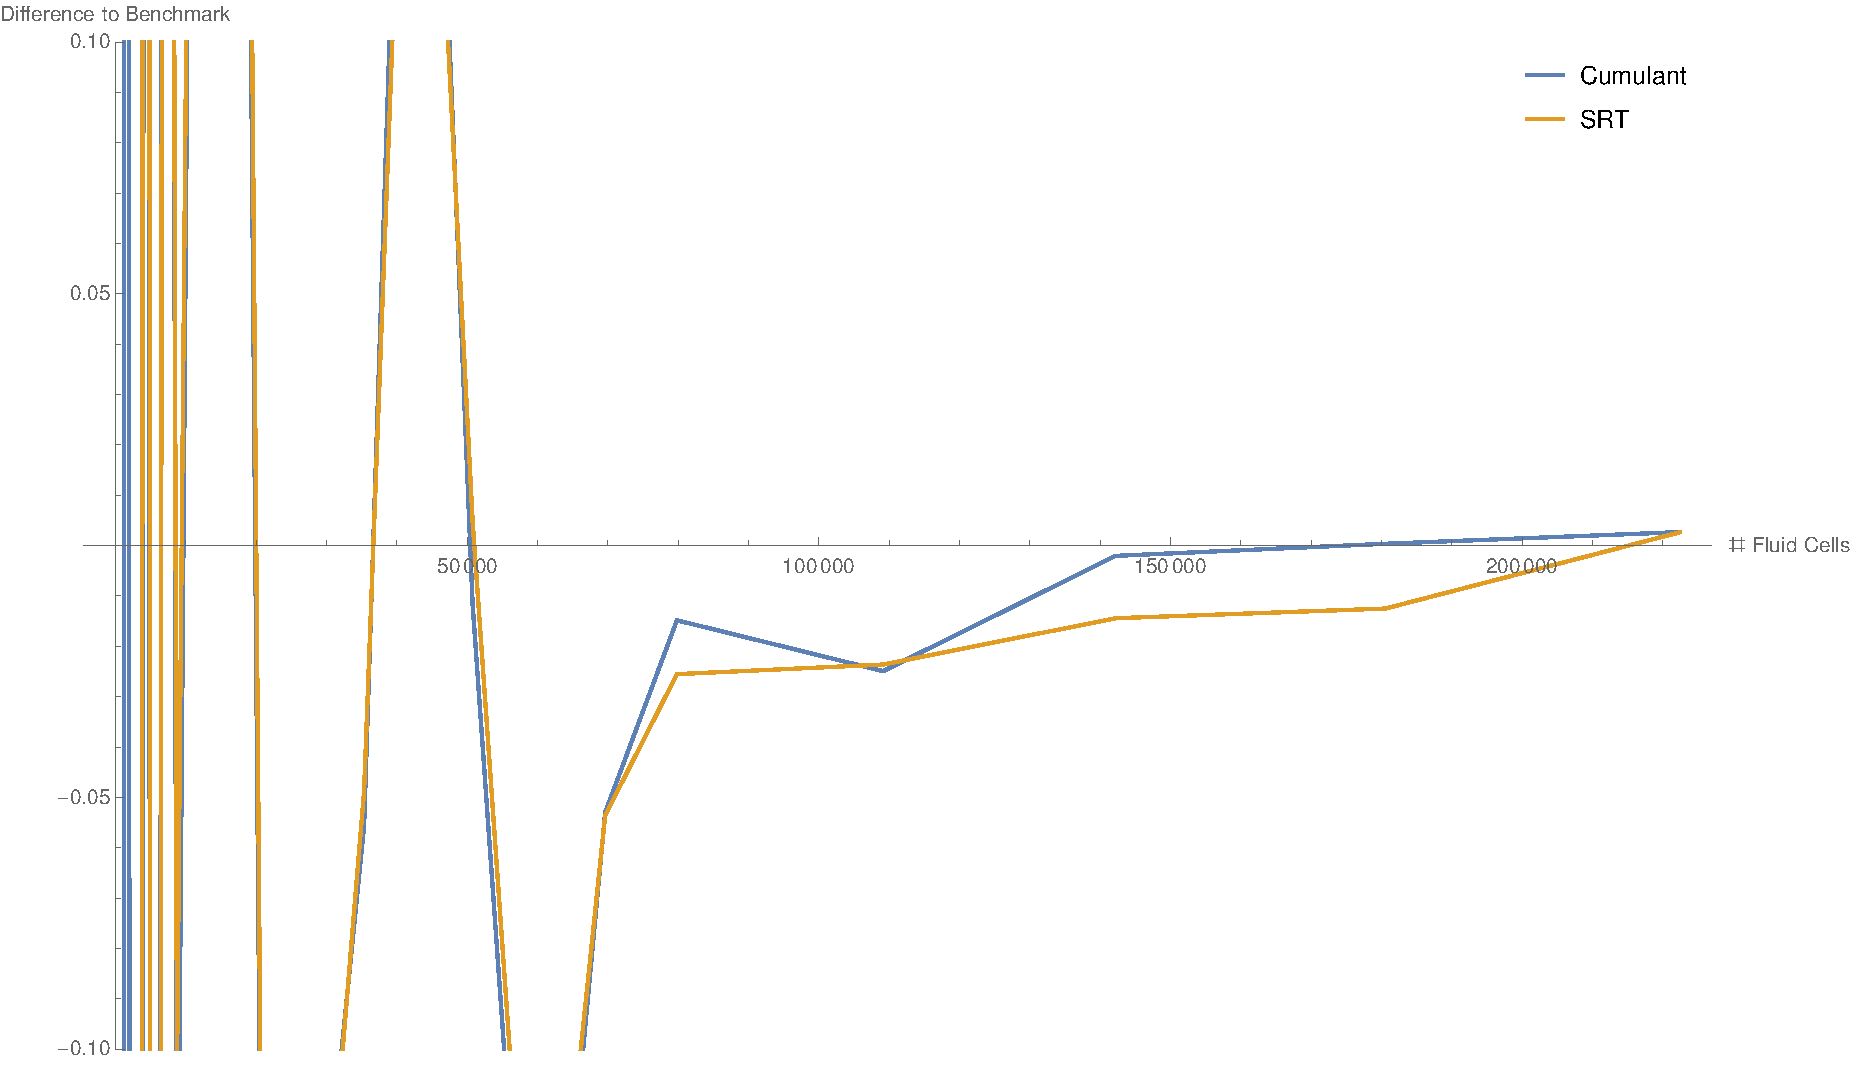
\includegraphics[width=\linewidth]{../figures/schaeferTurekLift_nrFluidVsDiff.pdf} % chktex 11
  \caption{Difference between the lift force of a sphere in relation to the computational domain.}
\label{fig: schaefer turek nrFluidVsDiff}
\end{figure}

Going over to the actual computation results, we find the situation depicted in Figure~\ref{fig: schaefer turek nrFluidVsDiff}.
The x-Axis is chosen to depict the number of fluid cells, the y-Axis is centered around $0.0110$, the value achieved with the biggest resolution in~\cite{schafer1996benchmark}.
At low resolutions, the lift is quite unsteady, presumably caused by the still bad approximation of the cylinder.
Going to the larger resolution, the Cumulants are converging faster than \gls{srt} to the benchmark result.

\begin{figure}
\centering
\begin{subfigure}{.48\textwidth}
  \centering
  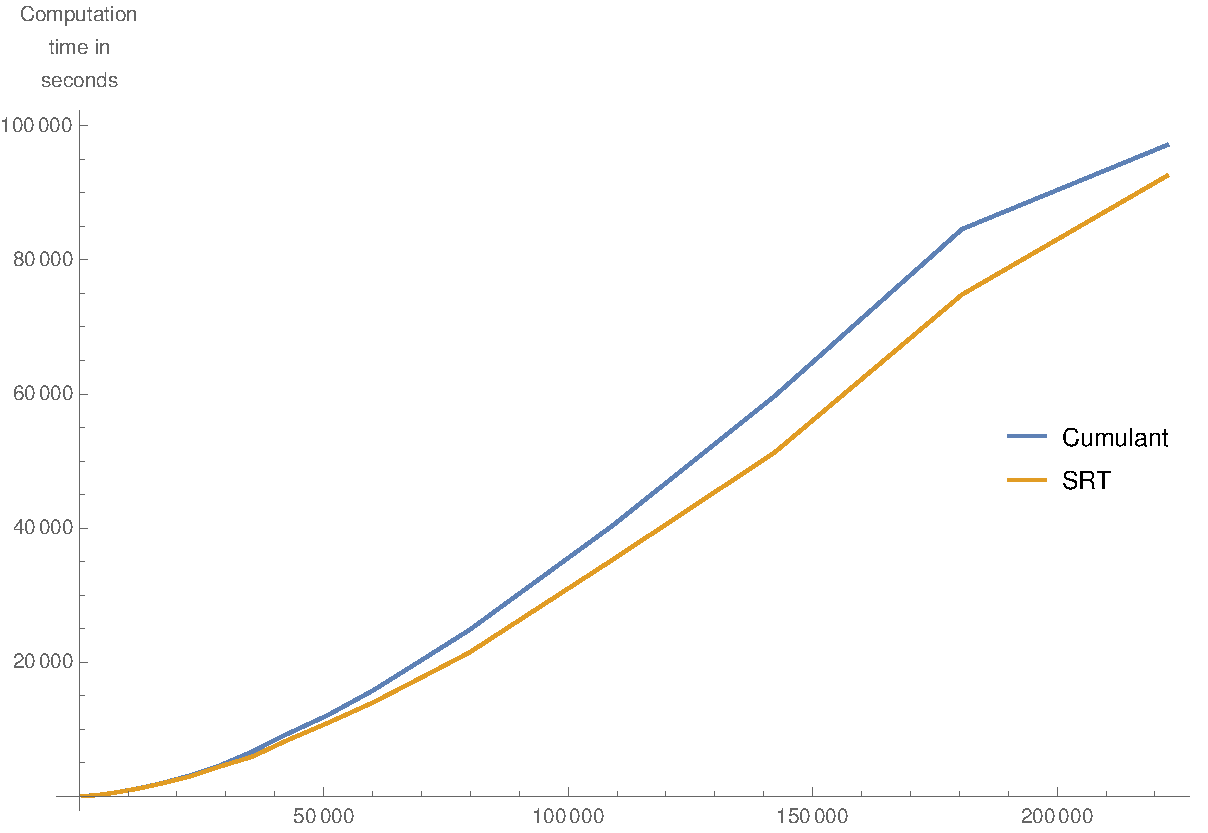
\includegraphics[width=\linewidth]{../figures/schaeferTurekLift_domainVsTime.pdf} % chktex 11
  \caption{Difference in computation time for Cumulants and SRT.}
\label{fig: schaefer turek domain vs time}
\end{subfigure}\hfill
\begin{subfigure}{.48\textwidth}
  \centering
  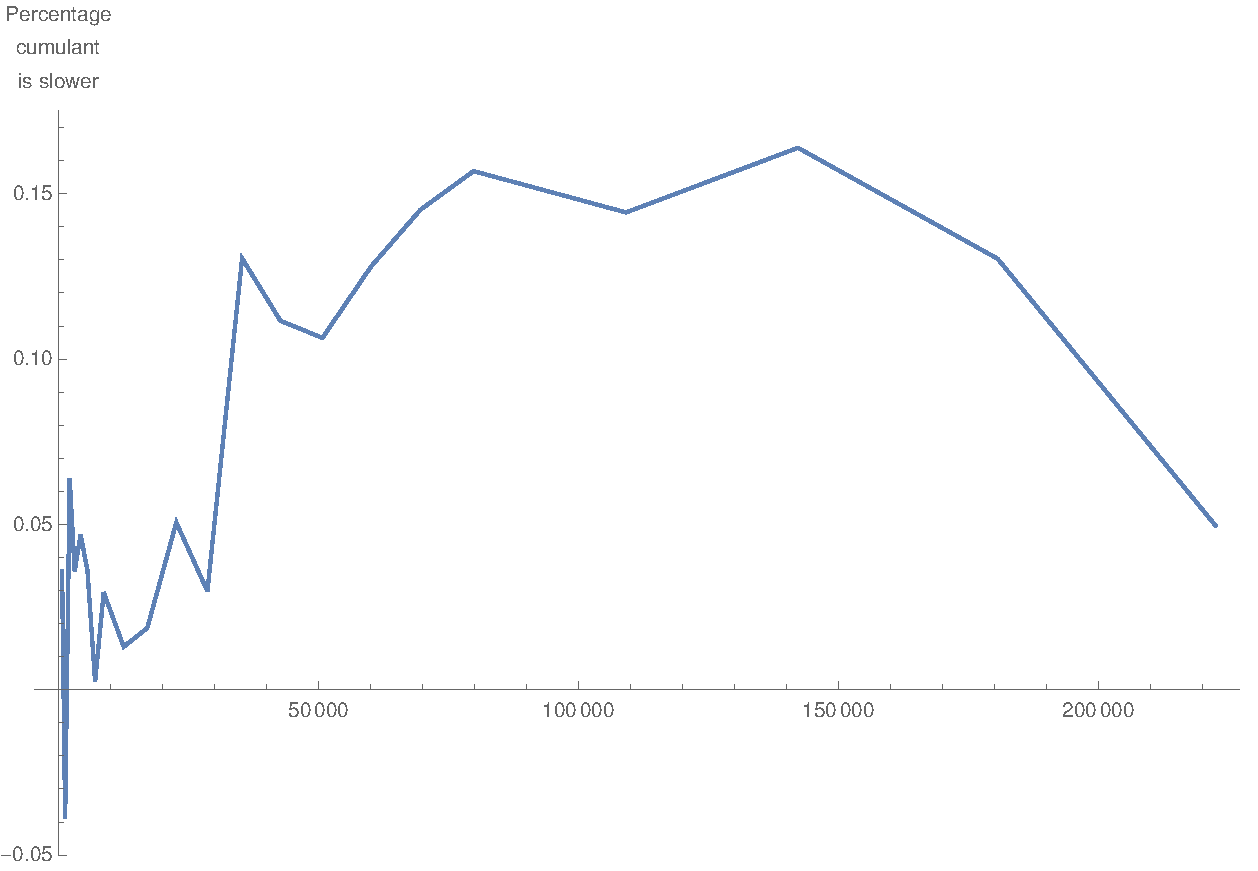
\includegraphics[width=\linewidth]{../figures/schaeferTurekLift_performanceGap.pdf} % chktex 11
  \caption{Percentage of additional time needed for Cumulant versus SRT.}
\label{fig: schaefer turek time percentage}
\end{subfigure}
\caption{Analysis of the difference in computation time. X-Axis is both times the number of fluid cells.}
\label{fig: time analysis cumulant vs SRT}
\end{figure}

This all sounds well, but we don't know yet if we sacrifice a whole lot of performance and thus just compare apples with oranges.
Figure~\ref{fig: time analysis cumulant vs SRT} wants to shed a bit of light onto this topic, analyzing the different runtimes.
We see that the cumulant method is indeed a bit slower, around $10-15\%$ to be more precise, which is not all that bad concerning how much transformation work has to be done.

Nevertheless, we have to tr eat this not just with a bit of caution, but a whole lot.
The implementation of both methods was done conscientious to not introduce major pitfalls and slowdowns.
It cannot be ruled out though, that one method allows for more low level optimizations\footnote{Be it multithreading, vectorization or just algebraic restructuring.} than the other, tilting the result.
However, a recent experimental implementation of the Cumulants in the highly optimized \href{http://walberla.net/index.html}{waLBerla}\footnote{widely applicable Lattice Boltzmann from Erlangen} showed a drop in MLUPs\footnote{Mega-lattice-updates per second} of about $50\%$ when compared to the native SRT, which is honestly quite amazing for a comparison to an unoptimized code.

\begin{figure}
  \centering
  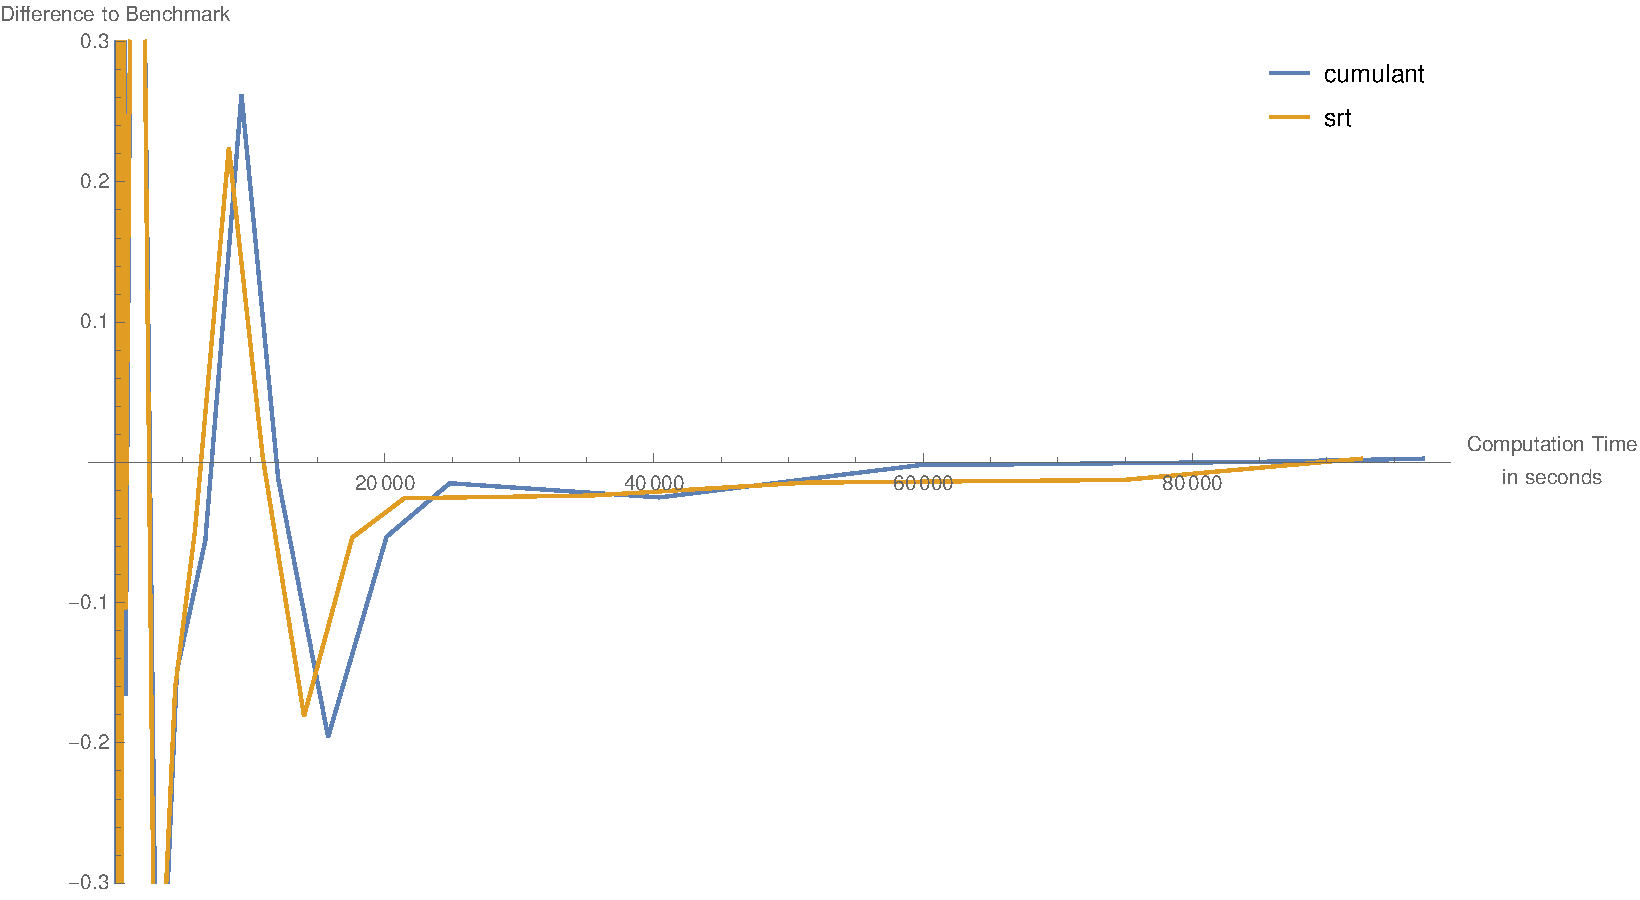
\includegraphics[width=\linewidth]{../figures/schaeferTurekLift_timeDifference.pdf} % chktex 11
  \caption{Difference between the lift force of a sphere in relation to the computational time.}
\label{fig: schaefer turek time difference}
\end{figure}

So, indeed it is reasonable to compare the methods with their runtimes, which was done in Figure~\ref{fig: schaefer turek time difference}.
Even here, the cumulant method features a much earlier convergence to the final result, despite the performance drop.


We can conclude, that the cumulant LBM is feasible if not superior to SRT even at low Reynolds numbers.
What's left is the analysis if cumulants also hold their promise if we crank the Reynolds number up.
